% Adapted from elsarticle-template-harv.tex supplied in resources/elsarticle.
% The Elsevier class and bibliography style retain their original licences.
\documentclass[final,3p,a4paper,authoryear]{elsarticle}

\usepackage[T1]{fontenc}
\usepackage{iftex}
\ifPDFTeX
  \usepackage[utf8]{inputenc}
\fi
% English is LaTeX's default language; no additional language package is needed.
\usepackage{lmodern}
\usepackage{amsmath,amssymb}
\usepackage{booktabs,tabularx,array}
\usepackage{float,placeins}
\usepackage{microtype}
\usepackage{xurl}
\usepackage[hidelinks,unicode]{hyperref}
\biboptions{authoryear,round}
\setlength{\emergencystretch}{2em}
\newcolumntype{Y}{>{\raggedright\arraybackslash}X}
\journal{Fil rouge Project -- AI and Healthcare}
\myfooter[C]{Fil rouge Project -- Working draft -- \today}
\abstracttitle{Abstract}
\keywordtitle{Keywords}

\begin{document}
% Outline item 1 is the Elsevier front matter.
\pdfbookmark[1]{1. Title, Abstract and Keywords}{frontmatter}
\begin{frontmatter}
\title{Operating Room Planning: Comparing Metaheuristics and Coupling
Optimisation with Reactive Simulation}
\author{Racha Bahlak}
\author{Thomas Casanova}
\author{Mathys Cornuaud}
\author{Virna Lissi Martinez Sanchez}
\author{Youri Pon-Drouet}
\author{Kau{\~a} Ribeiro de Sousa}

\begin{abstract}
Operating room planning must coordinate limited capacity while procedure
and hospital stay durations remain uncertain. This report connects a
historical-data audit, predictive modelling, five metaheuristics and execution
simulation. It distinguishes an aggregate session-and-bed model from a
minute-resolution room model coupled with Mesa. In the length-of-stay study,
changing session granularity alters algorithm rankings; the hybrid attains
the lowest mean cost among four split-session configurations, with a 5.70\%
gap to an overload lower bound under unequal search budgets. Upper-endpoint
stay estimates do not consistently reduce scenario-mean cost. The separate
room campaign comprises 144 initial plans replayed in 576 static/reactive,
closure/no-closure executions. All five searches reach the exact initial
allocation optimum on a seven-case fixture, but predicted improvements do
not guarantee better execution. Across 144 closure pairs, reactive planning
increases completions in 16, ties in 83 and reduces them in 45. A separate
1152-execution median/oracle comparison shows that perfect duration information
can increase throughput while also increasing overtime. These findings support
joint assessment of completions, overtime and computation rather than a
universal method ranking. Prediction matching, target conventions, cohort
selection, fixed sequencing and limited workload replication qualify the
results. Learned room-duration models and downstream resources require
further end-to-end evaluation.
\end{abstract}

\begin{keyword}
Operating room planning \sep Scheduling \sep Metaheuristics
\sep Hybrid optimisation \sep Simulation \sep Rescheduling
\end{keyword}
\end{frontmatter}

% Keep the outline numbering: front matter is item 1, Introduction is item 2.
\setcounter{section}{1}
\section{Introduction}
\label{sec:introduction}

\subsection{Context and motivation}

Operating room planning coordinates limited surgical capacity with clinical
teams, equipment and postoperative care. Decision horizon, patient pathway,
resources and performance criteria define distinct scheduling problems
\citep{cardoen2010,guerriero2011}. Improving room utilisation can shift pressure
to downstream units, which motivates integrated resource planning
\citep{rachuba2026}. Duration uncertainty adds a second difficulty: a schedule
built from estimates may execute differently, with delays, overtime or cases
unable to start \citep{denton2007}. These outcomes require separate metrics;
utilisation alone cannot summarise performance \citep{schouten2023}.

The Fil rouge AI and Healthcare project investigates this problem using
historical surgical activity. Its organisational motivation is to move from
calendar-driven booking towards capacity-aware admission and intervention
date recommendations \citep{group2026dataaudit}. The present experiments
address components of that ambition rather than a complete admission system.
One model assigns patients to multi-day operating sessions and penalises
session overload, bed demand and imbalance. A second assigns a daily workload
to rooms and evaluates minute-resolution execution in Mesa. It includes
turnover and temporary closures but excludes beds, staffing and speciality
compatibility. Their objective values are not directly comparable.

\subsection{Research question and positioning}

The research question is: \emph{with common information and evaluation rules,
how do operating room metaheuristics compare, and do improvements in predicted
schedule quality survive execution under duration deviations and temporary
room unavailability?}

Exact methods, metaheuristics and predictive--prescriptive pipelines are
already established in the literature \citep{fei2010,vieira2025,lex2025}.
Our contribution is a reproducible comparison with explicit representation,
information and resource assumptions. In the room experiments, every method
uses a shared decoder that fixes within-room order by increasing predicted
duration. Realised durations remain hidden during ordinary planning. Thus,
the study compares allocation search and execution policies within that
representation, not unrestricted surgical sequencing.

\subsection{Contributions and report organisation}

The report brings together three experimental contributions:
\begin{enumerate}
\item Five searches---simulated annealing, tabu search, a genetic algorithm,
      hybrid Tabu--Simulated Annealing and ant colony optimisation---compared
      with a greedy baseline and a small exactly enumerable room reference.
\item Static and closure-triggered reactive Mesa execution from shared
      initial schedules, plus a separate median/oracle duration comparison.
\item A length-of-stay (LOS) study linking learned estimates to session
      planning, with paired uncertainty scenarios and granularity sensitivity.
\end{enumerate}
The room campaign controls per-request fitness calls, whereas the LOS
campaign retains unequal source budgets. The hybrid search combines tabu
selection with annealing acceptance; simulation coupling instead evaluates
schedules during execution. Neither form of hybridisation implies clinical
validation or a universal best method.

The literature review and problem description establish scope.
Sections~\ref{sec:formulation}--\ref{sec:experimental-design} present the
formulations, methods and protocols; Sections~\ref{sec:results}
and~\ref{sec:discussion} report and interpret the evidence, followed by the
conclusion. The eleven-part structure keeps each experimental contribution
within these common sections.

\section{Literature Review}
\label{sec:literature-review}

This focused review covers decision levels, exact and approximate methods,
hybridisation and evaluation under uncertainty. It draws on accessible
reviews, methodological papers and retrospective studies; it is not an
exhaustive systematic review. Comparisons concern modelling choices and
evidence rather than a cross-study algorithm ranking.

\subsection{Planning, assignment and sequencing}

Operating room decisions range from strategic capacity to tactical session
allocation and operational case scheduling \citep{cardoen2010,guerriero2011}.
Choosing a date or session does not determine the within-day sequence.
\citet{alamin2025} review deterministic and uncertain formulations, while
\citet{wang2021} distinguish outpatient and inpatient scheduling. That
distinction matters when same-day discharge and overnight stays create
different downstream requirements.

Resource scope changes the problem. \citet{fei2010} separate weekly planning
from daily scheduling with recovery capacity, and \citet{rachuba2026} examine
integrated hospital planning. \citet{carter2024} smooth ward demand through
adjusted surgical activity; \citet{shehadeh2026} use distributionally robust
optimisation for assignment, sequencing and scheduling with uncertain surgery
and downstream stays. These formulations motivate resource integration,
but require information absent from a room-only dataset.

Duration targets must also remain distinct. Room occupancy, surgical
procedure time, turnover and hospital LOS measure different resource uses.
\citet{dupre2025} investigate room occupancy and LOS in emergency surgery;
neither target definition nor predictive performance transfers automatically
to elective planning. Our session-and-bed model and minute-resolution room
model consequently retain separate assumptions and objectives.

\subsection{Exact methods and interpretation of bounds}

Exact methods seek a model-specific optimum and may provide bounds when
interrupted. \citet{cardoen2009} use branch-and-price for day-care sequencing
with recovery resources and multiple criteria. In contrast, \citet{fei2010}
formulate planning as set partitioning but solve it with a column-generation
heuristic before hybrid genetic daily scheduling. An integer formulation
does not by itself certify the resulting solution.

Exhaustive enumeration is useful for small verification instances. With $n$
cases and $m$ rooms, the allocation space contains $m^n$ elements. The gap
$C(s)-C^\star$ is an optimality gap only when $C^\star$ is certified for the
same objective and decoder. An overload-based lower bound can support a bound
gap without proving optimality; a best-known value supports neither claim.
Even an exact predicted optimum does not certify performance under hidden
execution durations.

\subsection{Heuristics and metaheuristics}

Constructive rules provide fast baselines and initial incumbents.
Metaheuristics modify or rebuild these assignments under a finite budget,
with mechanisms that must be interpreted alongside representation and
feasibility handling.

\emph{Simulated annealing} accepts a cost increase $\Delta C>0$ with
probability $\exp(-\Delta C/T)$ as temperature decreases
\citep{kirkpatrick1983}. Temperature is therefore sensitive to objective
scale. \emph{Tabu search} uses move memory and aspiration to guide exploration
beyond local improvement \citep{glover1989}; sampled-neighbour count and
memory length affect both trajectory and effort.

\emph{Genetic algorithms} evolve populations through selection, crossover
and mutation. Their behaviour depends on encoding, repair and incumbent
retention. Surgical examples include \citet{fei2010} and the biased random-key
framework of \citet{vieira2025}. A generation cannot be equated with one
iteration of a single-solution method. \emph{Ant colony optimisation}
constructs solutions using heuristic desirability and pheromone memory
\citep{dorigo1996}. This foundational reference establishes the mechanism,
not hospital-specific superiority. In our allocation adaptation, favouring
a lightly loaded room is only a construction rule; the decoder must enforce
temporal feasibility.

Initial solutions, neighbourhoods, parameter settings and stopping criteria
are needed to explain differences between these methods. Equal fitness-call
budgets control one measure of effort, but candidate construction and
processing costs still differ; runtime must be reported separately.

\subsection{Hybrid approaches and a shared decoder}

Hybridisation can combine search mechanisms or connect distinct modelling
stages. \citet{fei2010} combine planning decomposition and daily search;
\citet{vieira2025} separate a random-key representation from deterministic
schedule decoding. The latter provides a useful comparison for a common
decoder, although our encoding and constraints differ.

The project's Tabu--Simulated Annealing hybrid selects candidates through
tabu memory and applies annealing acceptance. Any benefit requires comparison
with both components under stated budgets and repeated seeds. A lower cost
obtained with more evaluations does not isolate hybridisation itself.

Simulation coupling addresses a different question: whether decisions retain
value when execution diverges from planning assumptions
\citep{guerriero2011,rachuba2026}. Our search evaluates a predicted decoder
cost; Mesa executes the accepted plan and requests replanning at observed
availability events. It does not repeatedly simulate every search candidate.
Reactive policies may consume several request budgets, which must be included
in total effort.

Predictive--prescriptive hybrids add another stage. \citet{ahmadian2025}
combine a neural network with metaheuristics for operating rooms and
post-anaesthesia care under uncertain durations. \citet{kayvanfar2027},
published online in 2026 and assigned to a 2027 volume, connect estimation
with robust multi-resource optimisation. These studies motivate integration
but do not establish that one predictor or solver will dominate in our
simpler models.

\subsection{Prediction, uncertainty and realised performance}

\citet{merghani2025} review machine learning in operating room management,
supporting comparison of nonlinear models with simple historical references.
\citet{dupre2025} report residual uncertainty and speciality differences in
room-occupancy and LOS prediction. Predictive accuracy therefore requires
its own assessment, including temporal validation, calibration and tail errors.

\citet{lex2025} combine duration prediction with elective orthopaedic
optimisation and identify trade-offs between overtime and underutilisation.
\citet{lex2026} study a related single-centre arthroplasty pipeline. These
retrospective designs show how prediction can inform scheduling, while
transfer to other pathways and clinical settings remains conditional.

Prediction and scheduling must respect information timing. Encoders,
imputation and category grouping should use training data; realised durations
remain outcomes, not ordinary solver inputs. An explicit oracle scenario
changes that information boundary and must be labelled separately. A lower
prediction error or predicted objective does not necessarily improve every
operational metric, as the diversity reviewed by \citet{schouten2023} makes
clear. Completion, overtime, delay and resource use remain complementary.

\subsection{Positioning of the present study}

Table~\ref{tab:positioning} summarises the methodological comparisons.
Our contribution is a common experimental interface with explicit limits:
allocation search uses fixed sequencing, session penalties differ from the
room objective, and uncertainty scenarios differ from reactive execution.

\begin{table}[htbp]
\centering\small
\caption{Selected literature and its relevance to the experimental design.
The studies use different resources and are not interchangeable benchmarks.}
\label{tab:positioning}
\begin{tabularx}{\linewidth}{@{}lYY@{}}
\toprule
Study & Relevant approach & Comparison limit \\
\midrule
\citet{cardoen2009} & Exact day-care sequencing. & Richer recovery-resource model. \\
\citet{fei2010} & Weekly planning and hybrid daily scheduling. & Different decomposition and constraints. \\
\citet{vieira2025} & Searches sharing a decoder. & Different representation and search mechanisms. \\
\citet{dupre2025} & Room-occupancy and LOS prediction. & Emergency-surgery cohort and targets. \\
\citet{lex2025,lex2026} & Prediction followed by schedule optimisation. & Single-centre retrospective evidence. \\
\citet{rachuba2026} & Integrated hospital planning. & Broader scope than either project model. \\
\bottomrule
\end{tabularx}
\end{table}

\section{Problem Description}
\label{sec:problem-description}

\subsection{Decision setting and modelling scope}

Two complementary models assign a given workload to available capacity.
The aggregate model assigns patients to speciality sessions over several days
and approximates bed demand. The operational model assigns a daily workload
to rooms and evaluates execution in Mesa. They share search mechanisms but
have different decision spaces and objective scales. Static/reactive policy
comparisons concern the operational model.

An operational instance specifies cases, room count, opening hours, turnover
and an optional temporary closure. Rooms and calendars are experimental
assumptions rather than reconstructed hospital resources. All cases are ready
at opening. Days are independent: unstarted cases are counted, without
carryover, new arrivals or clinical prioritisation. The model evaluates a
fixed workload rather than a multi-day waiting list.

\subsection{Cases and available information}

Each case has a local identifier, procedure category and positive predicted
room-occupancy duration. A separate realised duration determines execution
and remains hidden from ordinary scheduling. Historical entry times define
observed occupancy but do not impose new-schedule release times or ordering.
The room baseline uses 2019--2021 procedure medians and a global fallback
for groups with fewer than ten observations; 2022 supplies evaluation cases.
Invalid dates and missing, zero or nonpositive clock intervals are excluded,
without interpreting exit-before-entry as overnight surgery. Durations round
up to integer minutes. Section~\ref{sec:room-design} reports selection counts.

At replanning, visible inputs are statuses, the accepted plan, estimated room
availability and revealed closures. For an ongoing case, availability uses
its predicted finish or at least the next minute if that prediction has
elapsed, followed by turnover. Hidden actual finish is not supplied. The
explicit oracle experiment instead substitutes realised occupancy estimates
while preserving workloads and resources.

\subsection{Aggregate sessions and bed demand}

A patient has speciality, operating minutes and stay days; a session has
speciality, day and minute capacity. The decision assigns each patient to a
session, without a start time or within-session sequence. Search options use
matching speciality when available, otherwise all sessions. This fallback
is computational and does not establish clinical compatibility.

Session load sums assigned durations. Bed occupancy counts the surgery day
through that day plus supplied LOS, inclusively, truncated to the planning
horizon. A zero-day stay therefore occupies one day. The model has a single
aggregate bed capacity, without existing occupants, bed types or explicit
admission/discharge processes. Session excess, bed excess and workload
standard deviation incur soft penalties; returned plans may exceed capacity.
The EDA adapter constructs sessions and derives a speciality proxy from codes,
requiring clinical confirmation. Historical durations are not out-of-sample
predictions unless a separate validated predictor supplies them.

\subsection{Room allocation and operational constraints}

Rooms are interchangeable: the operational model excludes beds, staff,
equipment and speciality eligibility. A solution allocates waiting cases to
rooms. The shared decoder orders each room's cases by increasing predicted
duration, breaking ties by local ID, then computes starts from current time,
opening, estimated availability and known closures. Sequence is fixed by
this rule rather than searched independently.

Every accepted schedule covers each case exactly once as assigned or
explicitly unassigned. Waiting assignments use integer starts and predicted
durations, respect availability and avoid predicted occupancy/turnover
overlap. Cases unable to start strictly before closing become unassigned,
but may be reconsidered at a later replan. Closing prohibits new starts,
not late finishes; required turnover contributes to overtime.

A closure blocks starts from its beginning up to reopening, without
interrupting ongoing non-preemptive work. Reassignment does not change realised
duration. Actual occupancy and turnover guard execution against conflicts
when predictions are optimistic. Planned starts remain lower bounds: cases
do not start early after an unexpectedly short predecessor unless replanned.

\subsection{Disruptions and rescheduling}

Static and reactive policies share one saved initial plan. Static execution
retains room assignments and order, allowing starts to slip when resources
remain occupied or closed. Reactive execution requests a plan at closure and
reopening. The closure is revealed when it begins, including its end time;
duration overruns alone do not trigger replanning.

Only waiting cases may change. Running/completed commitments remain fixed,
and the common validator checks coverage, resources, timing and consistency
with the current state. A failed replan retains the accepted plan; failed
initial planning leaves cases unassigned. Minute steps process completions
and turnover, availability changes, state synchronisation, optional replanning
and eligible starts. Simulated time pauses during solving, so measured
runtime is not itself an imposed patient delay.

\subsection{Objectives and performance criteria}

The room objective prioritises predicted unstarted waiting cases, then
overtime including turnover, then changed waiting decisions. Changes include
room/start revisions and assigned/unassigned transitions; they are inactive
at initial planning. Section~\ref{sec:room-formulation} formalises these
priorities. The aggregate model instead weights session excess, excess
bed-days and imbalance; raw costs cannot be compared across models.

Execution measures completed/unstarted cases, overtime, utilisation, delay
and revisions. Utilisation counts actual occupancy within opening hours,
excluding turnover, divided by configured room-hours; closure does not reduce
that denominator. Overtime sums post-closing occupancy and turnover over
rooms, excluding idle time. Start delay is relative to the initial plan and
measured only for completed cases with an initial assignment, requiring its
own denominator. Revisions count decision changes across replans, potentially
counting a case more than once. Fitness calls, solver time and request counts
measure effort. These definitions support interpretation within the model;
emergency arrivals, clinical urgency, staff constraints and downstream
congestion remain outside its operational scope.

\section{Mathematical Formulation}
\label{sec:formulation}

\subsection{Sets, parameters and assignment decisions}

For the aggregate model, let $I$ be the cases, $J$ the available sessions,
and $D=\{0,\ldots,H-1\}$ the planning days. Case $i$ has operating duration
$p_i$ and supplied integer stay $\ell_i$; session $j$ has day $d_j$, capacity
$c_j$ and speciality $a_j$. Let $J_i$ be the eligible session positions for
case $i$. The implementation uses matching speciality sessions when available,
otherwise all sessions; this fallback is a modelling limitation rather than
clinical authorisation. Let $b$ denote the constant aggregate bed capacity.

The binary variable $x_{ij}$ equals one if case $i$ is assigned to session
$j$. Each case receives exactly one eligible assignment:
\begin{equation}
 \sum_{j\in J_i}x_{ij}=1\quad(i\in I),\qquad
 x_{ij}\in\{0,1\}\quad(j\in J_i).
\end{equation}
The native solution dictionary stores the selected session's positional index,
not its external identifier. Capacity excess is penalised rather than ruled
out by a hard feasibility constraint.

Session load and bed occupancy on day $t$ are
\begin{align}
 L_j(x)&=\sum_{i:j\in J_i}p_i x_{ij},\\
 B_t(x;\ell)&=\sum_{i\in I}\sum_{j\in J_i}
 x_{ij}\,\mathbf{1}\{d_j\leq t\leq d_j+\ell_i\},\qquad t\in D.
\end{align}
Writing $[z]_+=\max(0,z)$, define
\begin{align}
 O_{\mathrm{session}}(x)&=\sum_{j\in J}[L_j(x)-c_j]_+,\\
 O_{\mathrm{bed}}(x;\ell)&=\sum_{t\in D}[B_t(x;\ell)-b]_+,\\
 \sigma_{\mathrm{load}}(x)&=\sqrt{\frac{1}{|J|}
 \sum_{j\in J}(L_j(x)-\overline L(x))^2},\qquad
 \overline L(x)=\frac{1}{|J|}\sum_{j\in J}L_j(x).
\end{align}
These definitions use all sessions, including empty ones, and the population
standard deviation used by the implementation. They describe the objective
evaluated by the search; no exact mathematical-programming solve is claimed.

\subsection{LOS planning objective and occupancy convention}

The LOS bridge links EDA cases to the predictor described in
Section~\ref{sec:data-prediction}. The point prediction and upper interval
endpoint define two planning instances. Operating durations remain historical
room-occupancy values; only LOS is varied in this study. The optimisation
cost is the existing session-model cost,
\begin{equation}
 C(x;\ell)=5\,O_{\mathrm{session}}(x)
          +3\,O_{\mathrm{bed}}(x;\ell)
          +0.05\,\sigma_{\mathrm{load}}(x),
 \label{eq:los-cost}
\end{equation}
Here $x$ is the assignment and $\ell$ the supplied stay vector. Fitness
is $-C$; reported costs are minimised. The weights are model-specific,
without monetary or clinical calibration. Bed counting includes surgery day
and the next $\ell_i$ days, clipped to the horizon. This differs from the
predictor's inclusive admission-to-discharge target and requires reconciliation;
preoperative admissions and existing occupants are not reconstructed.

\subsection{Operational room allocation and deterministic decoding}
\label{sec:room-formulation}

At decision time $t$, let $W$ be the waiting cases, $\mathcal R$ the rooms,
$N=|W|$, $[a,b)$ the opening window, $\tau$ the turnover time and $A_r$
the estimated availability of room $r$. Case $i$ has integer predicted
occupancy $p_i>0$. Running and completed assignments form a fixed set $F$.
The search chooses binary allocations $y_{ir}$ satisfying
\begin{equation}
 \sum_{r\in\mathcal R}y_{ir}=1\quad(i\in W),\qquad y_{ir}\in\{0,1\}.
\end{equation}
All rooms are eligible. Allocation does not guarantee that a case can start:
the decoder may return it explicitly unassigned.

Let $h_r(v)$ return the first minute at or after $v$ outside any currently
known start-blocking closure of room $r$. For each room, order its allocated
cases by $(p_i,\text{local ID}_i)$. Initialise $v_r=\max(t,a,A_r)$, then
compute $s_i=h_r(v_r)$. If $s_i<b$, accept the assignment and update
$v_r=s_i+p_i+\tau$; otherwise mark the case unassigned without advancing
$v_r$. Restore $F$ unchanged. This recurrence fixes the sequencing rule and
ensures predicted non-overlap with turnover; it does not optimise permutations.
Starts must satisfy $s_i\geq\max(t,a,A_r)$ and avoid known closures. Finishes
may exceed $b$. Future closures are absent until revealed by execution.

Write $D(y)$ for the decoded schedule and $W_A(y)$ for its assigned waiting
cases. Let $q_i(y)$ denote the complete room/start/duration assignment,
or the unassigned symbol, and let $q_i^0$ denote the accepted decision.
The request-level components are
\begin{align}
 U(y)&=N-|W_A(y)|,\\
 O(y)&=\sum_{i\in W_A(y)}[s_i+p_i+\tau-b]_+,\\
 R(y)&=\sum_{i\in W}\mathbf{1}\{q_i(y)\ne q_i^0\},
 \qquad B=\sum_{i\in W}(p_i+\tau).
\end{align}
At initial planning, set $R=0$. The implemented minimisation objective is
\begin{equation}
 C_{\mathrm{room}}(y)=U(y)+\frac{O(y)+R(y)/(N+1)}{B+1},
 \qquad f(y)=-C_{\mathrm{room}}(y).
 \label{eq:room-cost}
\end{equation}
Since starts precede closing, $O\leq B$; also $R\leq N$. The fractional
term is less than one, so an additional unstarted case dominates every
possible overtime/change improvement. Overtime uses integer minutes, and
$R/(N+1)<1$, so one minute dominates all changes. This encodes the intended
lexicographic priorities without clinically calibrated trade-off weights.
Fixed activity's overtime is constant within a request and excluded from
this score; execution metrics include it.

The admissible schedules must cover each case exactly once as assigned or
unassigned, retain $F$, and pass the common temporal validator. Enumeration
on a small instance certifies the best cost only among allocations decoded
by this rule. It does not certify optimal execution with hidden durations,
an optimal independent sequence, or an optimum across objectives. Different
workloads or duration modes change $B$, so raw normalised costs are not a
cross-instance performance scale.


\section{Proposed Hybrid Optimization Approach}
\label{sec:hybrid-approach}

\subsection{Combining tabu memory and simulated annealing}

The aggregate-model hybrid combines candidate ranking and short-term tabu
memory with a Metropolis acceptance rule. This description follows
\texttt{tabu\_simulated\_annealing} in the project implementation. It searches
the same assignment representation and fitness function as the comparison
methods, so improvements are evaluated using Equation~\ref{eq:los-cost}.
Tabu memory discourages recently recorded moves, while temperature-dependent
acceptance permits escape from a local improvement path.

\begin{enumerate}
\item Generate a random assignment, evaluate fitness $f=-C$, and initialise
      the incumbent best, an empty bounded tabu list and temperature $T_0$.
\item At each iteration, sample a neighbourhood, evaluate its assignments,
      and sort candidates by decreasing fitness.
\item Select the best candidate whose move is not tabu or whose fitness
      exceeds the best recorded fitness (aspiration). If none qualifies,
      the implementation uses the highest-ranked sampled candidate.
\item With $\Delta=f_{\mathrm{candidate}}-f_{\mathrm{current}}$, accept when
      $\Delta\geq0$ or with probability
      $\exp(\Delta/\max(T,10^{-9}))$ otherwise. On acceptance, record the
      move in tabu memory and update the best solution if improved.
\item Set $T\leftarrow\alpha T$, repeat until the iteration budget is used,
      and return the best recorded assignment and convergence history.
\end{enumerate}

The function defaults are 400 iterations, a tabu list of size 20, 15 sampled
neighbours per iteration, $T_0=20$ and $\alpha=0.97$. These are implementation
defaults, not a claim that every archived experiment used identical settings.
The comparisons retain each source campaign's parameter choices and stopping
rules; Section~\ref{sec:experimental-design} explains the resulting budget
limitations. Temperature is expressed on the fitness scale, so changing
objective weights can also change acceptance behaviour.

\subsection{Prediction interface and execution coupling}

Point and upper-endpoint LOS predictions provide alternative parameter
vectors $\ell$ to the same aggregate scheduler; their construction is given
in Section~\ref{sec:data-prediction}. Prediction does not replace the search
or change its assignment representation. The present LOS campaign freezes
the resulting schedules before scenario evaluation.

\subsection{Shared search interface and coupled parameter profile}
\label{sec:room-approach}

The room adapter reuses the five searches on waiting-case-to-room allocations
and evaluates each through the decoder and Equation~\ref{eq:room-cost}.
Reassignment and swap moves operate on this common space. At opening, a
greedy baseline inserts cases by increasing prediction into the earliest
available room. At replanning, the incumbent retains room choices from the
accepted plan and greedily inserts previously unassigned cases before decoding
against current availability. Local searches start from this incumbent;
GA includes it in the population and ACO retains it as the initial best.
Keeping the best evaluated candidate protects predicted request cost, while
execution can still deteriorate under duration error.

\begin{table}[htbp]
\centering\small
\caption{Coupled room-study settings. Iteration ceilings are raised so the
common fitness-call budget controls nontrivial searches. These fixed settings
are not the outcome of a tuning experiment.}
\label{tab:room-settings}
\begin{tabularx}{\linewidth}{@{}lY@{}}
\toprule
Method & Parameters \\
\midrule
SA & $T_0=1$, cooling $0.95$. \\
Tabu & Memory 20, 15 sampled neighbours. \\
GA & Population 40, crossover $0.8$, mutation $0.08$, elitism. \\
Hybrid & Memory 20, 15 neighbours, $T_0=1$, cooling $0.97$. \\
ACO & 15 ants, $\alpha=1$, $\beta=2$, evaporation $0.3$, deposit scale 1. \\
\bottomrule
\end{tabularx}
\end{table}

The room profile adapts both annealing temperatures to its normalised cost;
it must not be confused with the aggregate hybrid's $T_0=20$ default. ACO
constructs room assignments with probabilities proportional to
$\tau_{ir}^{\alpha}\eta_r^{\beta}$, where
$\eta_r=(1+L_r/c_r)^{-1}$ uses accumulated predicted load and remaining
capacity. This construction heuristic excludes turnover; complete candidates
are assessed by the common decoder. Pheromone evaporates by a factor $0.7$
per iteration, and the best ant's assignments receive $1/(1+C_{\mathrm{room}})$.
Pheromone is reinitialised for each request.

\subsection{Mesa execution and proposal acceptance}
\label{sec:coupling}

One Mesa agent represents a patient episode with waiting, running and
completed states; rooms are capacity resources. Coordination is centralised:
agents do not negotiate schedules or run their own optimisers. The execution
loop is as follows:
\begin{enumerate}
\item Build a request from the observable state, predictions and fixed
      running/completed assignments; omit hidden realised durations.
\item Obtain an allocation from the scheduler, decode it and check coverage,
      timing, turnover, known closures and preservation of fixed work.
\item Accept only a feasible proposal based on the current state version.
      A new state invalidates stale proposals; failed requests retain the
      accepted plan, or an all-unassigned plan if initial planning fails.
\item Advance one simulated minute: complete operations, release turnover,
      reveal closure/reopening, synchronise state and, under the reactive
      policy, request a new plan at those availability events.
\item Start eligible cases from the accepted schedule, subject to actual
      room occupancy, turnover, the start cutoff and closure guards.
\end{enumerate}
Static and reactive replays begin from the same saved initial schedule.
Duration overruns alone do not trigger replanning. A planned start remains
a lower bound until changed by an accepted replan. Execution duration is
unchanged by reassignment; ongoing work continues through a room closure.

Nontrivial searches run in separate processes with progress incumbents.
Budgets count initialisation and repeated fitness calls; cancellation/deadline
handling terminates and joins workers. A pre-search deadline may return a
validated incumbent with zero evaluations, labelled separately. Empty and
singleton requests use trivial/direct handling. Runtime includes startup and
communication; simulated time pauses during solving. This supports controlled
experiments, not a production response-time guarantee.


\section{Experimental Design}
\label{sec:experimental-design}

The aggregate LOS experiments incorporate Virna Lissi Mart\'inez S\'anchez's
report and structural sensitivity analysis \citep{martinez2026los}. The
room-execution campaigns are evaluated separately. Tables and figures are
regenerated from pinned aggregate results; original contributions retain
their attribution and source hashes.

\subsection{Data and predictive modelling}
\label{sec:data-prediction}

\subsubsection{Source data and targets}

The original workbook audit describes 14\,649 cases, 30 variables and
11\,108 patients; 2546 patients have repeated cases, up to nine per person
\citep{group2026dataaudit}. Interventions span 2 January 2019--30 December
2022, with one admission in 2018. Records cover demographics, clinical codes,
admission/discharge and pathway timestamps. They do not reconstruct reliable
room/session assignments, staffing, bed capacity, cancellations or rejected
dates. Experimental calendars and capacities are therefore assumptions.
Raw, cleaned, prediction-eligible and matched cohorts have different denominators.

Targets are inclusive admission-to-discharge LOS and room entry-to-exit
occupancy, distinct from incision-to-closure time. The audit found no exact
duplicate rows, but 2560 LOS values disagree with the date-derived target;
1884 recorded one-day stays span a night, and 31 recorded values resemble
Julian dates rather than durations. A one-day value alone cannot identify
ambulatory care. Zero clocks are treated as missing unless midnight is
confirmed: the audit reports 172 room-entry, 172 room-exit, 552 incision and
133 pre-anaesthesia zeros. Inverted intervals are not automatically repaired
by adding 24 hours. Section~\ref{sec:data-audit} retains further aggregate
checks; no original patient or professional identifiers are reproduced.

\subsubsection{Prediction time and evaluation}

Temporal and patient-disjoint evaluation measure different generalisation
settings. Imputation, encoding and category
rules use training data only. Historical medians, MAE, tail errors and
calibration provide complementary references. Features must be available
at decision time: discharge and observed pathway durations are excluded;
planned diagnoses, procedures, anaesthesia and clinician information remain
conditional on local preoperative availability. A changed proposed date
also changes any date-derived predictor. The implemented notebook and room
baseline splits are distinguished below.

\subsubsection{LOS predictor and matching interface}

The contributor uses XGBoost \citep{chen2016} on $\log(1+\mathrm{LOS})$ and
reports test MAE 0.412 days, $R^2=0.789$ and 89.4\% coverage for a nominal
90\% interval with half-width 1.02 days \citep{martinez2026los}. Scheduling
CSVs do not independently verify these metrics. The bridge uses a fixed
half-width in the inductive confidence-prediction tradition
\citep{papadopoulos2002}.

Back-transformed predictions are floored at one day and matched by patient
key and normalised intervention date, averaging duplicate key-date predictions.
Reported match rates are 86.7\% for the small workload and 86.4\% for the
large one. Unmatched cases receive the median matched prediction in the
selected window, or three days if no match exists; this is not an independently
estimated training median. Point and interval endpoints are rounded for
planning. The HIGH/LOW flag thresholds regression output above four days
and is distinct from the contributor's separately evaluated risk classifier.

\subsection{LOS instances, benchmarks and scenarios}

The original campaign compares SA, tabu, the hybrid, GA and ACO on 45 cases
with 35 sessions over five dates and 420 cases with 210 sessions over
30 dates. Capacity is 480 minutes per speciality-day and 42 aggregate beds.
The large workload has a speciality requiring 15\,438 minutes against
14\,400 available, so unavoidable overload is at least 1038 minutes and the
weighted objective has lower bound 5190, without certifying its full optimum.

The structural campaign splits each daily session into two 240-minute
sessions, preserving total capacity and giving 420 sessions. It tests SA,
tabu, the hybrid and GA with mutation $1/n$, without ACO. Original GA uses
0.08; a separate sensitivity run tests $1/n$. Source stopping rules and
unequal computation are retained rather than interpreted as a common-budget
comparison.

For each method and seed, point-LOS and upper-endpoint schedules are frozen
and evaluated on 200 common scenarios. Ten seeds, 42--51, support the main
comparisons; paired SE uses ten seed-level upper-minus-point scenario means,
not 200 independent optimiser runs. Original noise is uniform in
$[-1.02,1.02]$ days around unrounded predictions, clipped at one day and
integer-rounded. Alternatives use symmetric bounded noise with stochastic
rounding and extended, rather than horizon-truncated, bed tracking. These
are sensitivity rules, not distributions implied by interval coverage.
Additional experiments vary bottleneck-speciality block load across
0.80, 0.93, 0.98 and 1.10 with five seeds, keeping 42 beds. Matched-only
analysis retains 363 cases and removes 57 fallback cases, changing demand.

\subsection{Room/Mesa cohorts and paired experiment matrix}
\label{sec:room-design}

The separate room study uses the cleaned workbook, not the raw audit's
14\,649-row denominator. Its saved manifest records 14\,507 source rows,
14\,434 usable episodes and 73 exclusions, all zero clock endpoints in that
file version. Duration medians are learned from 10\,800 valid 2019--2021
cases, with a ten-observation threshold per procedure and a 70-minute global
fallback. Evaluation uses 2022. This temporal split permits recurring patients, unlike the patient-disjoint
model-preprocessing partitions described below.

The first room campaign contains one seven-case fixture, three historical
days (3 January: 9 cases; 2 February: 15; 20 October: 25), and two generated
samples at each of 100 and 300 cases. The selected dates have no exclusions; the middle and largest workloads
follow valid daily case counts among such dates. Generated instances sample complete eligible 2022
rows with replacement, retaining procedure--duration associations but not
within-day dependence. Each workload uses six methods and solver seeds
0, 1 and 2. Its 144 initial plans are each replayed under static/reactive
policies and closure/no-closure scenarios: 576 executions, not 576 independent
hospital days \citep{group2026roomstudy}.

Historical and generated days open 08:00--17:00 with 15-minute turnover.
Historical workloads use two interchangeable rooms; room 1 forbids starts
10:00--12:00 in the closure scenario. The small fixture uses two rooms,
08:00--11:00 and a 09:00--10:00 closure. Initial plans do not know the future
closure. For generated workloads,
\begin{equation}
 |\mathcal R|=\max\!\left(1,
 \left\lceil\frac{\sum_i(p_i+\tau)}{(b-a)\rho}\right\rceil\right),
 \qquad\rho=1.1.
\end{equation}
The four samples therefore use 14, 15, 44 and 45 rooms. Integer rounding
changes achieved load. This is an overloaded target experiment, not a
light-load sensitivity campaign; a single closure also represents a smaller
capacity fraction as the room pool grows.

Each nontrivial request has 1000 fitness calls and a 60-second safety limit.
No deadline stops occur in the saved campaigns. The baseline performs no
search evaluations. Reactive execution may use two additional request
budgets, so policies do not receive equal total computation. Runtime includes worker startup and communication. The 100-case runs were
sequential and 300-case runs used four concurrent batches, limiting timing
comparisons. Manifests record Python 3.12.3, Mesa 3.5.1, dependency versions
and source fingerprints, including dirty-checkout provenance.

\subsection{Duration-information experiment and predictive interfaces}
\label{sec:duration-design}

A separate saved campaign repeats the same matrix in median and oracle modes,
providing 1152 executions from 288 initial plans. These median runs are a
rerun, not extra independent replications of the first campaign. Oracle
mode replaces only scheduling estimates with realised room-occupancy minutes.
Workloads, execution durations and resources are held fixed; generated room
counts are computed from the original medians before substitution. Initial
plans are recomputed across modes but shared within each mode's four execution
conditions. Future closures remain hidden. This is a perfect-information
reference under finite search and a fixed decoder, not an ML predictor or a
certified operational upper bound. Normalised objective costs change scale
between modes; comparisons therefore use completions and realised overtime.

The operating-duration model branch \citep{group2026durationmodel} validates
patient-disjoint chronological partitions, excludes calendar features by
default, separates selection from later patient-disjoint calibration, and
selects the fastest candidate within 0.2 minutes of the best validation MAE.
Test data are reserved for reporting. Its review labels older metric tables
as belonging to a previous protocol; those are not verified current-model
results. Neither the median nor oracle campaign evaluates a learned room
model within Mesa.

Both preprocessing notebooks use pre-2021 training, new-patient validation
in 2021 and new-patient testing from 2022, excluding later cases of patients
in earlier partitions. Split identifiers/dates remain audit metadata.
Target-derived fields and postoperative/discharge information are excluded
from predictors; clinical codes require confirmed preoperative availability.
These controls must survive model-to-scheduler integration.

\subsection{Verification and reproducible evidence}

The incorporated room tables are regenerated from pinned aggregate CSVs.
Checks enforce unique run keys, four replays per initial plan, case conservation,
paired mode coverage and equality of no-closure policy outcomes. An independent
review of all 576 primary and 1152 duration execution exports recomputes
occupancy and overtime and checks start windows, closures, turnover separation,
evaluation caps and shared initial schedules. All pass, with zero reported
coordinator/search failures, timeouts or deadline stops. Validation of the reviewed source snapshot ran 94 tests, with 92 passing
and two optional tests skipped. These
checks support implementation consistency; they do not validate clinical
assumptions or make solver-seed repetitions independent observations.


\subsection{Additional source-workbook audit details}
\label{sec:data-audit}

By admission year, the raw audit counts are 1 (2018), 3690 (2019),
3526 (2020), 3764 (2021) and 3668 (2022); intervention dates are in 2019--2022.
All interventions lie between admission and discharge in that audit, with
no missing date endpoints or discharge before admission. These checks retain the raw-audit denominator rather than that of the
cleaned room cohort.

\begin{table}[H]
\centering\small
\caption{Selected additional quality checks in the original workbook audit.
Timestamp comparisons exclude zero clocks and use their own valid-pair denominators.}
\label{tab:source-quality}
\begin{tabularx}{\linewidth}{@{}YY@{}}
\toprule
Check & Audit result \\
\midrule
Associated diagnosis fields 1--5 & Missingness 20.7\%, 43.2\%, 63.2\%, 77.1\%, 86.9\%. \\
Secondary procedure fields 2--4 & Missingness 7.3\%, 38.6\%, 66.0\%. \\
Anaesthesia / locoregional anaesthesia & Missingness 15.3\% / 37.1\%. \\
Room exit before entry & 0 of 14\,477 comparable pairs. \\
Room exit before incision / incision before entry & 4 / 42 of 14\,026 pairs. \\
Room entry / exit before pre-anaesthesia entry & 309 / 2 of 14\,442 pairs. \\
\bottomrule
\end{tabularx}
\end{table}

Administrative spreadsheet completeness therefore does not imply valid
clinical timing. Zero-coded endpoints and inverted intervals require explicit
handling, not an automatic 24-hour correction. High-cardinality coding
(617 principal diagnoses, 570 principal procedures and 1433 intervention-type
labels) motivates category harmonisation. The audit's coded-sex categories
require confirmation before interpretation. The full aggregate source audit,
including variable families, population summaries and detailed LOS discrepancy
counts, is preserved in the pinned contribution archive. No patient or
professional identifiers are reproduced.

% Keep audit tables inside Experimental Design.
\FloatBarrier
\section{Computational Results}
\label{sec:results}
% Prevent result tables from floating above their section heading.
\suppressfloats[t]

The first results concern the aggregate LOS study. The room/Mesa campaign
and its separate median/oracle comparison follow in
Sections~\ref{sec:room-results} and~\ref{sec:duration-results}. Each family
retains its own objective, workloads and experimental replication unit.

\subsection{Solution quality and computation time}

Table~\ref{tab:los-legacy} retains the original five-method comparison.
For the large workload, SA, tabu and the hybrid achieve mean nominal costs
near 5198--5207, close to the overload-based lower bound. Default GA has a
mean cost of 8569.4; changing its mutation probability to $1/n$ reduces this
to 5286.9 in the sensitivity comparison. Thus, the default result does not
establish an inherent weakness of genetic search. ACO reaches 5783.5 and
requires about 10.08 seconds, compared with 0.27 for SA and 0.33 for tabu.
These runtimes are measurements from the contributor's machine and campaign,
not hardware-independent guarantees. On the small instance, all five methods
have costs around 3.25--3.29, with no session or bed overload, so the instance
provides little discrimination between them.

% Generated by scripts/summarise_los_results.py; do not edit manually.
\begin{table}[tbp]
\centering
\small
\caption{Original five-method campaign: nominal cost for the large workload (mean $\pm$ SD, ten seeds), and planning time averaged over point and upper-bound modes. GA uses its default mutation probability here; ACO was not run in the later split-session campaign.}
\label{tab:los-legacy}
\begin{tabularx}{\textwidth}{@{}Yrrr@{}}
\toprule
Method & Large cost & Small (s) & Large (s) \\
\midrule
SA & $5206.7 \pm 26.2$ & 0.11 & 0.27 \\
Tabu & $5198.4 \pm 0.0$ & 0.13 & 0.33 \\
Hybrid & $5198.3 \pm 0.0$ & 0.21 & 0.53 \\
GA (default) & $8569.4 \pm 521.3$ & 0.28 & 0.87 \\
ACO & $5783.5 \pm 170.0$ & 0.99 & 10.08 \\
\bottomrule
\end{tabularx}
\end{table}


Table~\ref{tab:los-quality} and Figure~\ref{fig:los-granularity} compare
point-LOS planning across session structures. With one 480-minute session,
tabu and the hybrid have mean gaps of about 0.16\% to the lower bound,
compared with 0.32\% for SA and 1.87\% for tuned GA. With two 240-minute
sessions, the hybrid's mean cost is 5485.9, a 5.70\% gap, compared with
5892.3 for tabu, 6022.1 for SA and 7217.0 for tuned GA. The hybrid has the
lowest mean cost among the four methods tested in that configuration; this
comparison cannot establish its superiority to the untested ACO variant.

% Generated by scripts/summarise_los_results.py; do not edit manually.
\begin{table}[tbp]
\centering
\small
\caption{Large workload: point-LOS schedule cost (mean $\pm$ SD over ten seeds), gap to the session-overload lower bound of 5190, and mean planning time. These are gaps to a lower bound, not certified gaps to the true optimum.}
\label{tab:los-quality}
\begin{tabularx}{\textwidth}{@{}Yrrr@{}}
\toprule
Method & Cost & Bound gap & Time (s) \\
\midrule
\multicolumn{4}{@{}l}{\emph{One 480-minute session per speciality-day}} \\
SA & $5206.7 \pm 26.2$ & 0.32\% & 0.276 \\
Tabu & $5198.4 \pm 0.0$ & 0.16\% & 0.336 \\
Hybrid & $5198.3 \pm 0.0$ & 0.16\% & 0.543 \\
GA ($p_{\mathrm{mut}}=1/n$) & $5286.9 \pm 44.1$ & 1.87\% & 0.793 \\
\midrule
\multicolumn{4}{@{}l}{\emph{Two 240-minute sessions per speciality-day}} \\
SA & $6022.1 \pm 196.8$ & 16.03\% & 0.385 \\
Tabu & $5892.3 \pm 347.1$ & 13.53\% & 0.441 \\
Hybrid & $5485.9 \pm 115.1$ & 5.70\% & 0.755 \\
GA ($p_{\mathrm{mut}}=1/n$) & $7217.0 \pm 333.0$ & 39.06\% & 1.176 \\
\bottomrule
\end{tabularx}
\end{table}


\begin{figure}[tbp]
\centering
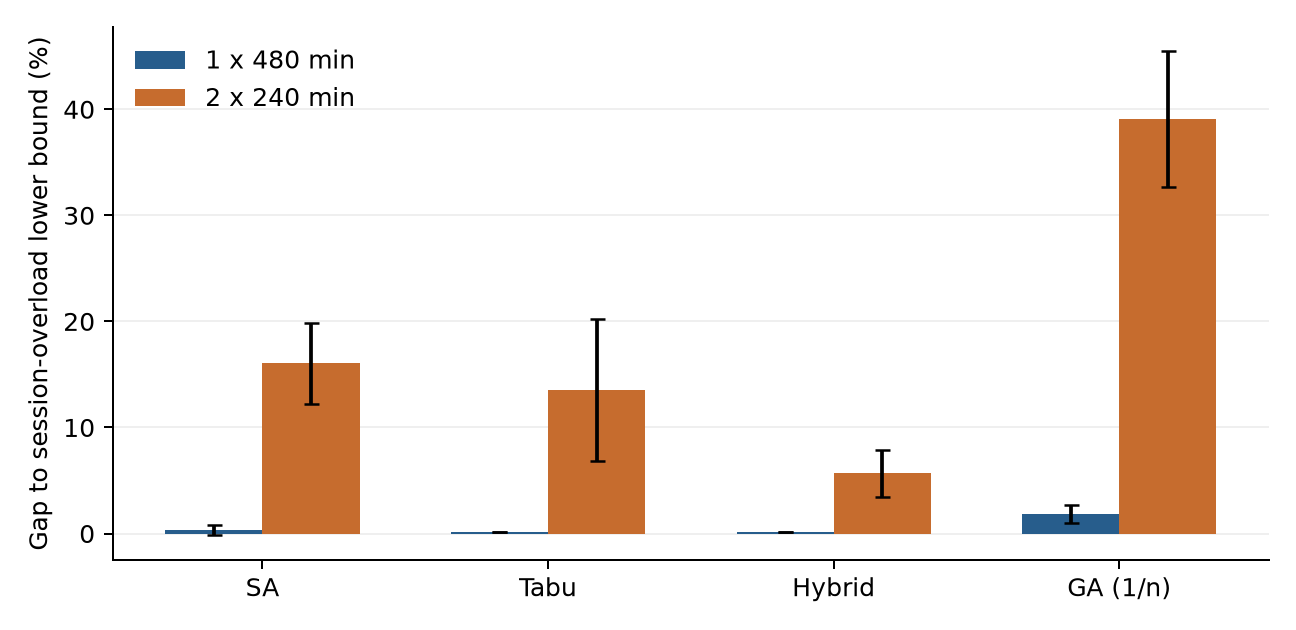
\includegraphics[width=0.88\linewidth]{figures/los-granularity.png}
\caption{Effect of session granularity on nominal schedule quality. Total
speciality-day capacity is unchanged. Bars show mean percentage gaps to the
5190 lower bound; error bars show SD across ten seeds.}
\label{fig:los-granularity}
\end{figure}

Splitting capacity changes the assignment landscape even though the total
number of available minutes is unchanged. The observed ranking therefore
depends on session granularity as well as the algorithm. The hybrid also
uses more computation: its mean point-planning runtime in the split-session
campaign is 0.755 seconds, versus 0.385 for SA and 0.441 for tabu. This is an instance-specific comparison under unequal computation;
the lower-bound gap does not prove optimality.

\subsection{LOS scenarios and upper-bound planning}

For the large workload, mean rounded nominal LOS is about 1.90 days. The
floor-noise scenarios average about 2.10 days, while the alternative symmetric
rule averages about 1.98 days. Clipping and differences between unrounded
predictions and rounded nominal inputs therefore change the mean as well
as variability. Under point planning, the original floor-noise evaluation
raises expected cost by about 109--115 for SA, tabu and the hybrid. Since
only LOS changes when a schedule is re-evaluated, this increase acts through
the bed term of Equation~\ref{eq:los-cost}; it is not deterioration in room
assignment itself.

The effect of upper-bound planning is best assessed using paired expected
costs rather than the increase relative to each schedule's own nominal
baseline. Table~\ref{tab:los-robustness} and
Figure~\ref{fig:los-uncertainty} retain the configuration and scenario labels
for this comparison. In the one-session configuration, upper-bound planning
increases scenario-mean cost by 68.4 for SA, 63.1 for tabu and 102.3 for the
hybrid. The source also reports lower dispersion, indicating a cost/predictability
trade-off.

% Generated by scripts/summarise_los_results.py; do not edit manually.
\begin{table}[tbp]
\centering
\small
\caption{Paired change in scenario-mean cost, upper-bound planning minus point planning (mean $\pm$ SE across ten seeds). Negative values favour upper-bound planning. Floor-noise scenarios and horizon-truncated bed tracking are used in both configurations.}
\label{tab:los-robustness}
\begin{tabularx}{\textwidth}{@{}Yrr@{}}
\toprule
Method & $1\times480$ min & $2\times240$ min \\
\midrule
SA & $+68.4 \pm 12.0$ & $-88.6 \pm 68.8$ \\
Tabu & $+63.1 \pm 12.9$ & $+31.3 \pm 87.6$ \\
Hybrid & $+102.3 \pm 7.9$ & $+9.1 \pm 34.1$ \\
GA ($p_{\mathrm{mut}}=1/n$) & $-12.0 \pm 19.6$ & $-98.4 \pm 167.8$ \\
\bottomrule
\end{tabularx}
\end{table}


\begin{figure}[tbp]
\centering
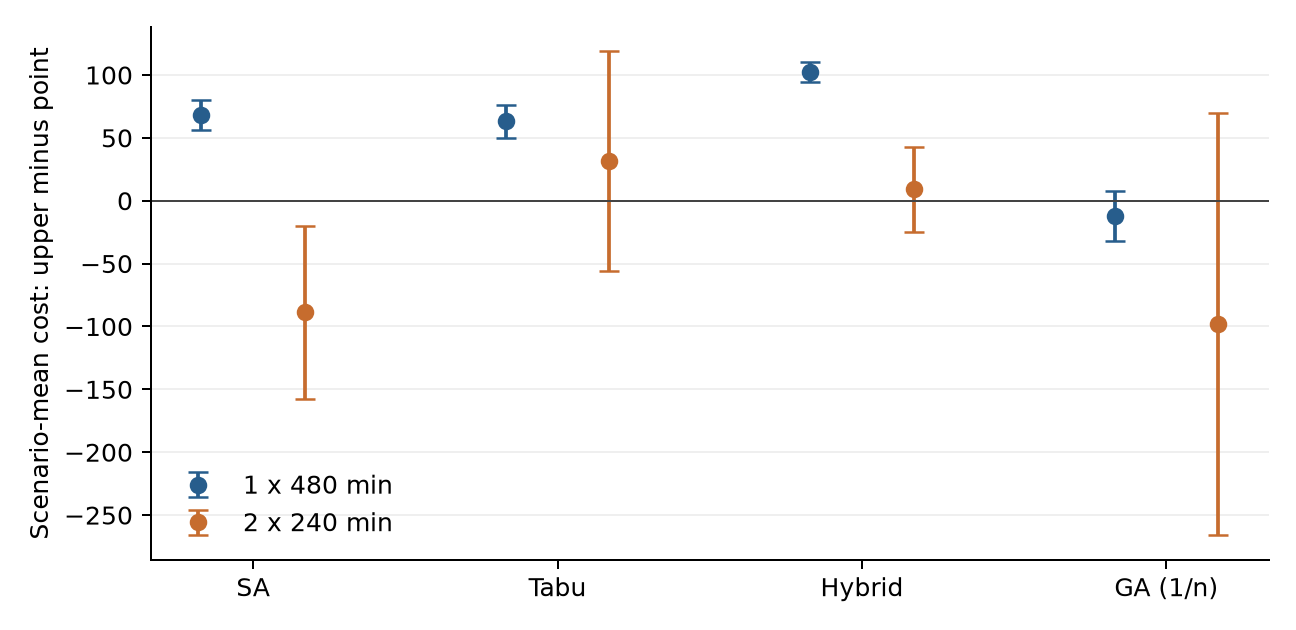
\includegraphics[width=0.88\linewidth]{figures/los-uncertainty.png}
\caption{Paired scenario-mean cost differences for upper-bound versus point
planning, using floor noise and horizon-truncated bed accounting. Error bars
are one SE across ten paired seeds, not confidence intervals. Negative values
favour upper-bound planning.}
\label{fig:los-uncertainty}
\end{figure}

The two-session results are less conclusive: paired differences are
$-88.6\pm68.8$ for SA, $31.3\pm87.6$ for tabu, $9.1\pm34.1$ for the hybrid
and $-98.4\pm167.8$ for tuned GA, expressed as mean $\pm$ SE. These results show a method-dependent effect with substantial uncertainty;
a uniform increase or benefit under this configuration is not established. More generally, a
small increase from a schedule's own baseline is not evidence of lower
absolute cost or protection from extreme failures. Scenario distributions,
horizon treatment and the cost baseline must remain explicit.

\subsection{Load, matching and horizon sensitivity}

Figure~\ref{fig:los-load} preserves the source study's load experiment with
an explicit axis definition. The varied quantity is operating-block load
for the bottleneck speciality, obtained by changing session capacity; the
figure does not establish a critical bed-utilisation threshold at 93\%.
The bed capacity is fixed and only four target block loads are examined.
Five seeds per load also limit the precision of comparisons.

\begin{figure}[tbp]
\centering
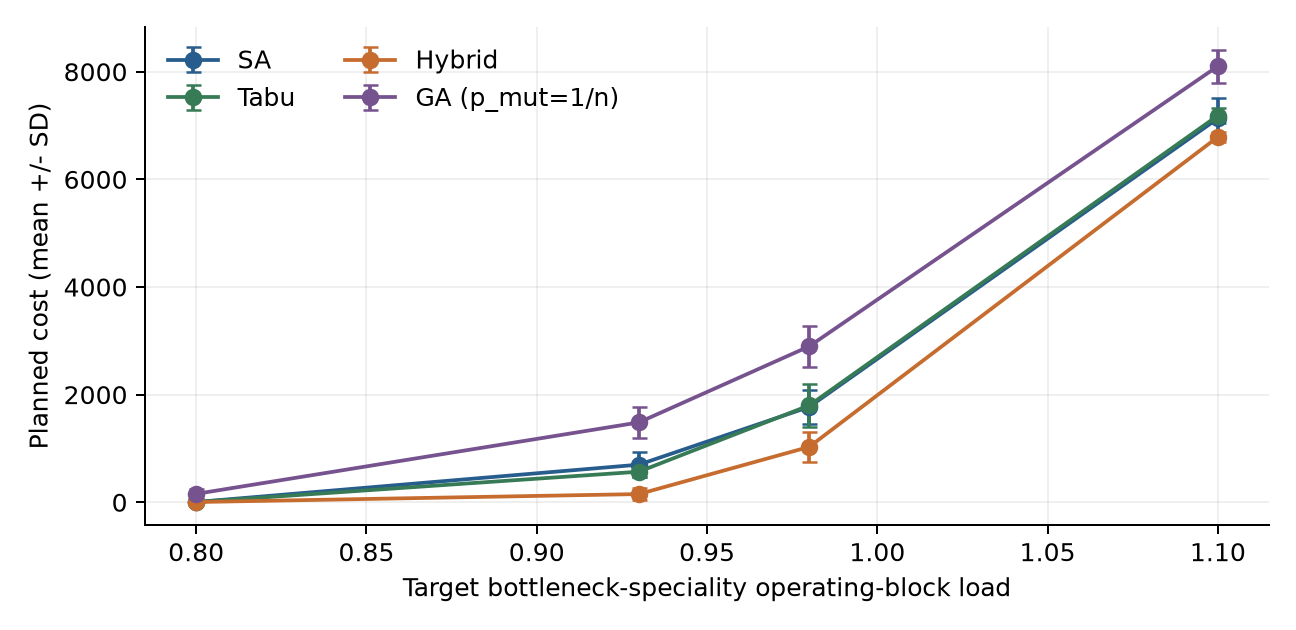
\includegraphics[width=0.88\linewidth]{figures/los-block-load.png}
\caption{Planned cost versus target operating-block load for the two-session
configuration. Points show means and error bars show SD over five seeds.
The horizontal axis is not measured bed utilisation.}
\label{fig:los-load}
\end{figure}

In the matched-only workload, the overload lower bound is zero. The hybrid
achieves zero session overload and a mean nominal cost of 7.13, consisting
of workload imbalance; tabu's mean cost is 7.65. Percentages relative to a
zero lower bound are undefined. Removing 57 cases changes demand as well
as prediction matching, so the improvement cannot be attributed solely to
better model linkage. The source also examines full-stay accounting because
horizon truncation can favour postponing patients towards the last days.
Extended accounting is a sensitivity analysis of frozen plans, not a claim
that the planning objective itself has been replaced.


% Finish the LOS floats before the room-study results.
\FloatBarrier
\subsection{Room allocation: exact reference and predicted search quality}
\label{sec:room-results}

The room fixture has seven predicted durations of 30--90 minutes in ten-minute
increments, two rooms and $2^7=128$ allocations. Enumeration gives $U=0$,
$O=165$ and $C_{\mathrm{room}}=0.313688$. Table~\ref{tab:room-exact} shows
that all five searches reach this optimum at every tested seed; the greedy
baseline has an absolute cost gap of 0.80038. This is a predicted allocation certificate only: without closure, hidden
durations leave mean completions at 5.67--6 of seven cases across methods.

\begin{table}[H]
\centering\small
\caption{Small room-allocation reference: absolute initial predicted-cost gaps, exact hits and mean initial solve time. Three seeds on one fixed seven-case fixture; baseline repeats are identical.}
\label{tab:room-exact}
\begin{tabular}{@{}lrrrr@{}}
\toprule
Method & Mean gap & Worst gap & Exact hits & Time (s) \\
\midrule
Baseline & 0.80038 & 0.80038 & 0/3 & 0.000 \\
SA & 0.00000 & 0.00000 & 3/3 & 0.523 \\
Tabu & 0.00000 & 0.00000 & 3/3 & 0.521 \\
GA & 0.00000 & 0.00000 & 3/3 & 0.523 \\
Hybrid & 0.00000 & 0.00000 & 3/3 & 0.538 \\
ACO & 0.00000 & 0.00000 & 3/3 & 0.574 \\
\bottomrule
\end{tabular}
\end{table}


Table~\ref{tab:room-initial} separates predicted initial quality from execution.
At 100 cases, SA, tabu and the hybrid reduce mean predicted overtime from
668.0 minutes for the baseline to 602.0. At 300 cases, tabu and the hybrid
reach 1905.5 versus 2195.0 for the baseline; SA reaches 1908.0. All retain
zero predicted unstarted cases. GA retains the incumbent at both sizes;
ACO improves it at 100 cases but not at 300. These rankings are specific to the tested budget.

\begin{table}[H]
\centering\small
\caption{Generated workloads: initial predicted unstarted count U, overtime OT and end-to-end solve time, averaged over six plans per method and size. These predicted quantities are distinct from execution outcomes. The 300-case campaign used four concurrent batches.}
\label{tab:room-initial}
\begin{tabular}{@{}rlrrr@{}}
\toprule
Cases & Method & Predicted U & Predicted OT & Time (s) \\
\midrule
100 & Baseline & 0.00 & 668.0 & 0.002 \\
100 & SA & 0.00 & 602.0 & 0.696 \\
100 & Tabu & 0.00 & 602.0 & 0.679 \\
100 & GA & 0.00 & 668.0 & 0.697 \\
100 & Hybrid & 0.00 & 602.0 & 0.682 \\
100 & ACO & 0.00 & 616.2 & 1.366 \\
300 & Baseline & 0.00 & 2195.0 & 0.009 \\
300 & SA & 0.00 & 1908.0 & 1.098 \\
300 & Tabu & 0.00 & 1905.5 & 1.107 \\
300 & GA & 0.00 & 2195.0 & 1.128 \\
300 & Hybrid & 0.00 & 1905.5 & 1.089 \\
300 & ACO & 0.00 & 2195.0 & 3.707 \\
\bottomrule
\end{tabular}
\end{table}


The mean initial time is approximately 0.68--0.70 seconds for the four
non-ACO searches at 100 cases, compared with 1.37 seconds for ACO. At
300 cases, corresponding means are approximately 1.09--1.13 and 3.71 seconds.
Baseline timing excludes a search worker. Per-candidate work differs, and
concurrent 300-case execution limits cross-size timing interpretation. Larger
room instances have no certified optimum or optimality gap.

\subsection{Static and reactive execution under room closure}

Historical outcomes vary by day (Table~\ref{tab:room-historical}). All methods
complete nine cases on 3 January under both policies, but reactive overtime
is higher. On 2 February, tabu and the hybrid move from 12.00 completed cases
and 158.7 overtime minutes under static execution to 11.33 and 108.0 under
reactive execution. Lower overtime here accompanies fewer completed cases.
On 20 October, all methods complete 16 of 25 cases under both policies, while
reactive overtime falls from 110 minutes to about 73.7--82.7. Day-level comparisons therefore matter.

\begin{table}[H]
\centering\small
\caption{Historical closure scenario: mean completed cases and realised overtime over three solver seeds per day. S = static; R = reactive. Each pair shares its initial plan. Overtime includes turnover and sums minutes over rooms.}
\label{tab:room-historical}
\begin{tabular}{@{}llrrrr@{}}
\toprule
Date & Method & Done S & Done R & OT S & OT R \\
\midrule
2022-01-03 & Baseline & 9.00 & 9.00 & 64.0 & 92.0 \\
2022-01-03 & SA & 9.00 & 9.00 & 7.3 & 44.7 \\
2022-01-03 & Tabu & 9.00 & 9.00 & 15.7 & 57.3 \\
2022-01-03 & GA & 9.00 & 9.00 & 61.0 & 95.0 \\
2022-01-03 & Hybrid & 9.00 & 9.00 & 15.7 & 57.3 \\
2022-01-03 & ACO & 9.00 & 9.00 & 10.3 & 41.0 \\
2022-02-02 & Baseline & 11.00 & 11.00 & 59.0 & 113.0 \\
2022-02-02 & SA & 11.67 & 11.33 & 135.3 & 109.3 \\
2022-02-02 & Tabu & 12.00 & 11.33 & 158.7 & 108.0 \\
2022-02-02 & GA & 11.67 & 11.00 & 115.0 & 68.0 \\
2022-02-02 & Hybrid & 12.00 & 11.33 & 158.7 & 108.0 \\
2022-02-02 & ACO & 11.67 & 11.33 & 154.7 & 121.3 \\
2022-10-20 & Baseline & 16.00 & 16.00 & 110.0 & 77.0 \\
2022-10-20 & SA & 16.00 & 16.00 & 110.0 & 74.0 \\
2022-10-20 & Tabu & 16.00 & 16.00 & 110.0 & 75.7 \\
2022-10-20 & GA & 16.00 & 16.00 & 110.0 & 73.7 \\
2022-10-20 & Hybrid & 16.00 & 16.00 & 110.0 & 75.7 \\
2022-10-20 & ACO & 16.00 & 16.00 & 110.0 & 82.7 \\
\bottomrule
\end{tabular}
\end{table}


The generated closure workloads also show mixed effects
(Table~\ref{tab:room-generated}). At 300 cases, baseline replanning raises
mean completions from 287.5 to 289.5 and overtime from 2838.0 to 3319.5
room-minutes. Tabu and the hybrid begin at 289.0 completions under static
execution and fall to 287.33 and 287.50 respectively when reactive. These
policy differences are conditional on each method's shared initial plan;
they do not compare methods from a common initial allocation.

\begin{table}[H]
\centering\small
\caption{Generated closure scenario: means over two sampled workloads and three solver seeds (six runs per cell). Resources are 14/15 rooms for 100 cases and 44/45 for 300 cases. OT is realised overtime including turnover, in room-minutes.}
\label{tab:room-generated}
\begin{tabular}{@{}rlrrrr@{}}
\toprule
Cases & Method & Done S & Done R & OT S & OT R \\
\midrule
100 & Baseline & 97.00 & 97.00 & 933.5 & 1022.0 \\
100 & SA & 96.67 & 96.17 & 952.5 & 958.5 \\
100 & Tabu & 96.50 & 95.67 & 876.0 & 856.0 \\
100 & GA & 97.00 & 96.33 & 933.5 & 971.7 \\
100 & Hybrid & 96.50 & 96.17 & 876.0 & 932.8 \\
100 & ACO & 96.33 & 96.00 & 902.5 & 976.0 \\
300 & Baseline & 287.50 & 289.50 & 2838.0 & 3319.5 \\
300 & SA & 287.33 & 286.33 & 2923.0 & 3028.5 \\
300 & Tabu & 289.00 & 287.33 & 3021.5 & 3140.5 \\
300 & GA & 287.50 & 286.00 & 2838.0 & 2974.5 \\
300 & Hybrid & 289.00 & 287.50 & 3021.5 & 3165.5 \\
300 & ACO & 287.50 & 285.17 & 2838.0 & 3000.5 \\
\bottomrule
\end{tabular}
\end{table}


Across all 144 closure pairs, reactive execution completes more cases in 16,
the same number in 83 and fewer in 45. Overtime falls in 64, ties in seven
and rises in 73. The counts include deterministic baseline repeats and are descriptive.
All no-closure static/reactive pairs have identical completion, overtime,
occupancy and total delay, as expected when no replanning trigger occurs.

\begin{figure}[H]
\centering
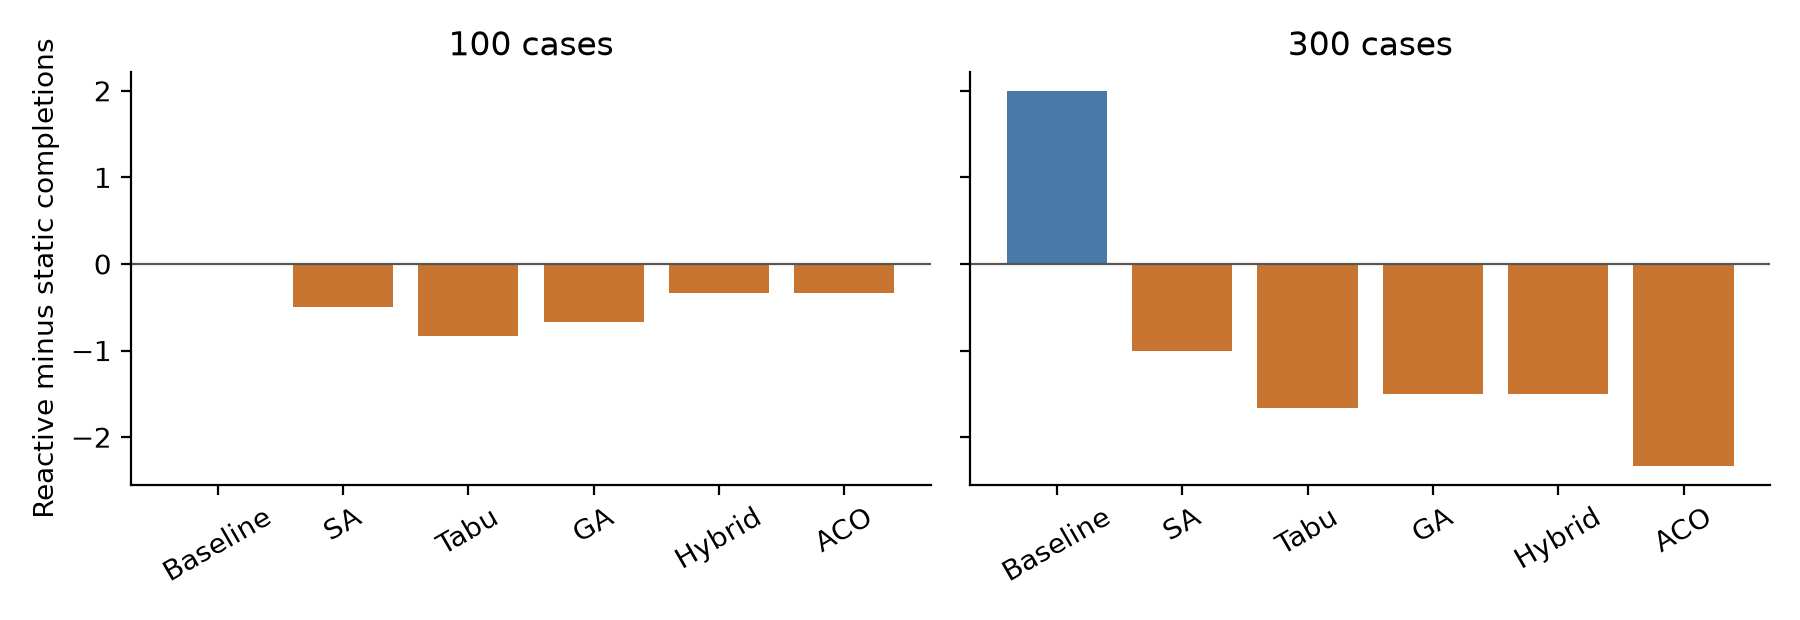
\includegraphics[width=0.95\linewidth]{figures/room-policy-differences.png}
\caption{Mean paired completion differences under closure in the primary
room campaign. Each bar averages two generated workloads and three solver
seeds; positive values favour reactive execution. No confidence intervals
or statistical superiority are claimed. Read alongside overtime in
Table~\ref{tab:room-generated}.}
\label{fig:room-policy}
\end{figure}

\subsection{Perfect duration information: a separate execution comparison}
\label{sec:duration-results}

Table~\ref{tab:room-duration} uses the separate median/oracle campaign,
restricting the displayed comparison to no-closure static execution so
neither disruption nor reactive replanning changes between modes. At 300
cases, oracle estimates allow all six methods to complete 300 cases on average,
compared with 287.5--289.17 under median estimates. Oracle overtime is
3590.5--3678.0 room-minutes, compared with 2779.0--2965.0: additional throughput
comes with more post-closing occupancy, consistent with the objective's
priority for case starts.

\begin{table}[H]
\centering\small
\caption{Separate duration-information campaign: no-closure static execution. M = historical-median estimates; O = oracle durations. Means use two workloads and three solver seeds. Resources and hidden outcomes are held fixed across modes; initial plans are recomputed. OT includes turnover.}
\label{tab:room-duration}
\begin{tabular}{@{}rlrrrr@{}}
\toprule
Cases & Method & Done M & Done O & OT M & OT O \\
\midrule
100 & Baseline & 97.50 & 99.50 & 922.0 & 886.0 \\
100 & SA & 97.17 & 100.00 & 942.7 & 908.5 \\
100 & Tabu & 97.17 & 100.00 & 874.7 & 908.5 \\
100 & GA & 97.50 & 99.50 & 922.0 & 883.3 \\
100 & Hybrid & 97.17 & 100.00 & 874.7 & 908.5 \\
100 & ACO & 97.17 & 100.00 & 908.5 & 927.5 \\
300 & Baseline & 287.50 & 300.00 & 2779.0 & 3678.0 \\
300 & SA & 288.00 & 300.00 & 2949.7 & 3590.5 \\
300 & Tabu & 289.17 & 300.00 & 2965.0 & 3590.5 \\
300 & GA & 287.50 & 300.00 & 2779.0 & 3678.0 \\
300 & Hybrid & 289.17 & 300.00 & 2965.0 & 3590.5 \\
300 & ACO & 287.50 & 300.00 & 2779.0 & 3678.0 \\
\bottomrule
\end{tabular}
\end{table}


At 100 cases, the four non-GA searches complete all 100 cases under oracle
estimates, whereas baseline and GA complete 99.5 on average. In the small
fixture, each metaheuristic completes all seven cases with 240 overtime
minutes under oracle information; the baseline still completes six with
105 minutes. Perfect information therefore does not compensate for every
search or representation restriction, nor does it necessarily lower overtime.
Duration substitution also changes ordering and search landscape. Learned
models require their own held-out end-to-end comparison; oracle gains do
not estimate their operational benefit.


% Keep result figures and tables inside Computational Results.
\FloatBarrier
\section{Discussion and Managerial Insights}
\label{sec:discussion}

\subsection{Prediction quality, allocation quality and execution performance}

The two study families support different conclusions. The LOS campaign links
learned stay estimates to session planning and shows that session granularity
and GA mutation settings can alter observed rankings. The room campaign
shows that reaching an exact predicted allocation optimum, or improving
predicted overtime on a larger instance, does not guarantee more completed
cases under hidden durations. Execution evaluates a different quantity from
the surrogate search score. The oracle comparison further shows that more
accurate duration information can increase throughput and overtime together
when the objective prioritises case starts. Prediction MAE, predicted cost,
completions and overtime should therefore be reported separately.

Reactive replanning supports every solver, yet produces gains, ties and
losses. It optimises the visible state with fixed sequencing and reacts only
to closure/reopening, rather than optimising future execution scenarios.
This is a plausible explanation for mixed effects, not evidence that
rescheduling is inherently harmful. Alternative triggers and sequencing
rules require separate experiments.

\subsection{Implications for planning and resource management}

Managers need to assess throughput and overtime jointly. On the 15-case
historical day, lower reactive overtime for tabu and the hybrid accompanies
fewer completed cases; on the 25-case day, overtime falls without changing
completion counts. A recommendation based on overtime alone would conflate
these outcomes. Delay also has a selected population: only completed cases
with an initial assignment contribute, so a method can change both the
average and its denominator. Utilisation excludes turnover and retains
closed room-hours in its denominator; it is not interchangeable with an
availability-adjusted utilisation measure.

Session structure is itself a planning choice: dividing unchanged minutes
into smaller blocks changes the assignment landscape. The LOS hybrid's
5.70\% lower-bound gap in the split-session experiment supports further
comparison under a common budget, not a universal recommendation. Point and
upper-endpoint LOS should remain explicit alternatives with cost and
variability trade-offs. Their relative value depends on workload, weights,
noise rules and bed-accounting conventions.

The capacity-aware date-recommendation ambition is only partially represented. Daily room
experiments allocate a fixed workload and do not propose admission dates,
carry a waiting list across days or enforce ward capacity. The aggregate
model represents beds but has no minute-level execution. Combining their
findings does not establish a validated end-to-end admission recommendation
system. Surgeon availability, staff, equipment, clinical priority and
pre-existing ward occupancy need their own data and constraints.

\subsection{Robustness, generalisation and remaining evidence gaps}

The room campaign uses three solver seeds and only three historical days,
plus two generated samples per size. Seeds repeat a workload and deterministic
baseline repetitions add no workload diversity. Generated rows retain
procedure--duration pairing but omit day-level correlations. The 1.1 target
load and single-room closure do not characterise light-load performance or
constant proportional disruption severity. Equal per-request evaluation
budgets differ from equal policy-wide computation; concurrent 300-case timing
and paused simulation time further limit operational latency conclusions.
Larger held-out workload samples, several loads and budgets, and alternative
disruption patterns are needed before claiming general superiority.

For LOS, a constant-width conformal interval does not capture patient-specific
heteroscedasticity; uniform in-interval noise omits outside-tail events and
clipping changes its mean. Coverage, target units and feature availability
require saved-model verification. About 14\% of cases lack matched predictions,
with fallback depending on the selected workload. Inclusive total LOS differs
from the optimiser's surgery-day-plus-stay occupancy convention; horizon
truncation omits downstream demand. The matched-only variant removes cases,
so its improvement cannot isolate matching quality.

Learned room-model evaluation must pin the current dataset, category mapping,
selected artefact and calibration sample, then provide held-out predictions
for the exact room-occupancy target. Existing median/oracle room experiments
and frozen-plan LOS scenarios do not measure that end-to-end benefit.

Implementation verification checks case conservation, resource consistency,
information boundaries and reproducible scoring. It does not establish
clinical validity. Multi-day ward dynamics, emergency arrivals, patient
priority, unrestricted sequencing, clinically confirmed resource eligibility
and prospective workflow evaluation remain scientific extensions, rather
than demonstrated capabilities of the campaigns reported here.

\section{Conclusion}
\label{sec:conclusion}

This report combines a historical-data audit, a predictive LOS interface,
five metaheuristics and a room-level simulation-optimisation framework.
It formalises separate session-and-bed and operational room objectives,
describes the shared decoder and acceptance loop, and retains the provenance
of each experimental contribution.

The LOS results show that session granularity can change algorithm rankings
at unchanged total capacity. The hybrid attains the lowest mean cost among
four split-session configurations, with a 5.70\% gap to an overload lower
bound under unequal search budgets. Upper-endpoint planning does not
consistently reduce scenario-mean cost. In the room campaign, all searches
reach the small fixture's exact initial allocation optimum, while larger
predicted improvements need not survive execution. Reactive scheduling
improves completions in 16 of 144 closure pairs, ties in 83 and worsens them
in 45. The separate oracle experiment illustrates that increased throughput
can require increased overtime even with perfect duration information.
These are descriptive findings under explicit modelling assumptions, not
a universal method ranking or evidence of clinical effectiveness.

Further work should reconcile LOS and bed-accounting conventions, evaluate
current learned room-duration models on held-out workloads, compare total
computation as well as per-request budgets, and vary loads, disruptions and
sequencing policies. Integrating ward dynamics, staff and clinical constraints
would connect the current experiments more closely to admission-date decision
support. Such extensions require additional data and validation; they are
not implied by the successful software integration.


\renewcommand{\bibsection}{\section{References}\label{sec:references}}
\begingroup
% Compact, readable reference leading avoids a one-entry overflow page.
\renewcommand{\bibfont}{\fontsize{8}{9}\selectfont}
\bibliographystyle{elsarticle-harv}
\bibliography{bibliography}
\endgroup
\end{document}
